\section{Introduction}
\label{sec:introduction}
Continual learning (CL) allows models to lean new skills while retaining prior knowledge, effectively mitigating catastrophic forgetting (CF)~\citep{mcclelland1995there, mccloskey1989catastrophic}. This capability is essential in dynamic real-world settings, where models must continuously adapt to evolving data while preserving previously acquired knowledge~\citep{zhang2023vqacl}. Despite significant advances in CL, most research has focused on unimodal tasks (\eg image classification)~\citep{wang2022dualprompt, wang2022continual, kirkpatrick2017overcoming, NEURIPS2023_15294ba2, marouf2024weightedensemblemodelsstrong, zhou2024expandable}.
However, real-world applications often require multimodal learning that integrates complex visual and textual reasoning. Visual Question Answering (VQA) stands as a representative multimodal task, requiring models to jointly interpret visual content and natural language. For instance, answering questions like ``\textit{What color is the car on the left?}'' or ``\textit{How many trucks are visible?}'' requires robust object recognition and a nuanced grasp of the linguistic query structure~\citep{zhang2023vqacl, schwenk2022okvqa, yang2022zero, cheng2023vindlu, Wang_2023_ICCV}.

\begin{figure}
    \centering
    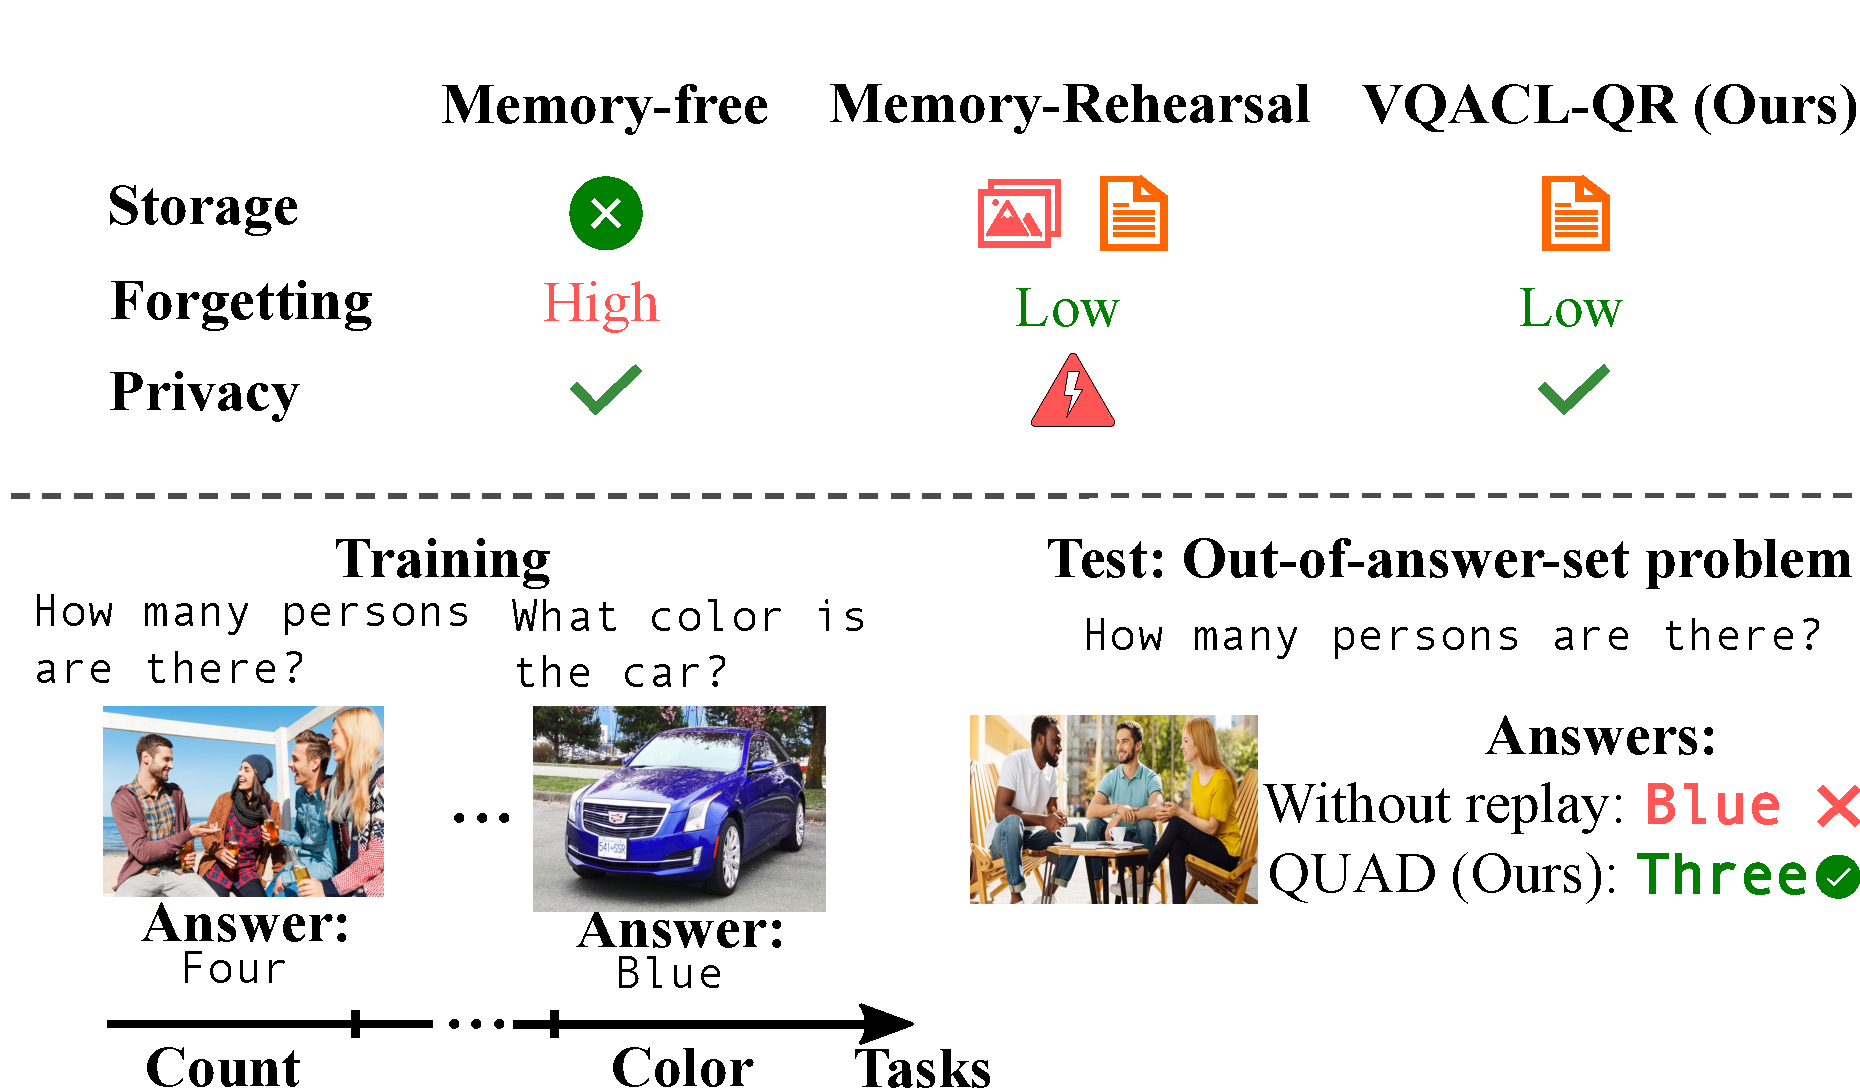
\includegraphics[width=\linewidth]{Figures/teaser2.pdf}
    \caption{Comparison of continual learning methods for Visual Question Answering (VQA) in terms of storage, forgetting, and privacy. \textbf{Memory-free} methods ensure privacy but suffer from high forgetting. \textbf{Memory-rehearsal} methods reduce forgetting but raise privacy concerns by storing sensitive images (\textit{e.g.} people's identities, car plates). Our approach \textbf{\qstmethodshort{}}, only stores questions and avoids image storage, preserving privacy while achieving low forgetting by leveraging question-based regularisation to effectively solve the out-of-answer set problem.}
    \label{fig.teaser}
\end{figure}
The emerging field of Visual Question Answering Continual Learning (VQACL)~\citep{zhang2023vqacl} focuses on enabling models to improve VQA performance iteratively by learning from a sequence of tasks without catastrophic forgetting. Unlike static pretrained multimodal models~\citep{liu2023llava, li2023blip2, agrawal2024pixtral12b} that rely on massive datasets and heavy computation, VQACL offers a more efficient and scalable alternative by allowing incremental adaptation without costly re-training~\cite{zhang2023vqacl, nikandrou2022task}. Research in VQACL is further driven by the broader scientific goal of developing multimodal agents that continuously improve their reasoning throughout deployment in a multimodal environments.
A key challenge in VQACL is balancing \textit{stability}—the preservation of past knowledge—and \textit{plasticity}—the ability to learn new information—across both visual and linguistic modalities~\citep{zhang2023vqacl, antol2015vqa}. This dual-modality requirement, combined with the need for generalisation ability, introduces additional complexity in learning. Models must retain visual and linguistic knowledge across tasks, while also generalizing to novel objects and unseen question types. For example, a model that masters counting vehicles should be able to transfer this counting capability to novel object categories, such as bicycles~\citep{greco-etal-2019-psycholinguistics}.

To achieve this balance, continual VQA methods rely on memory-based replay, where previously seen examples are stored and revisited to reinforce prior knowledge and mitigate forgetting~\citep{chaudhry2019tinyepisodicmemoriescontinual, Chaudhry2019er, Wan_2022_CVPR, zhang2023vqacl}. In VQACL, this necessitates storing full image-question pairs, which demands substantial memory resources, often amounting to thousands of samples per task (\eg 5000 samples in VQACL~\citep{zhang2023vqacl}). Storing visual data poses two core challenges. \emph{First}, it incurs high computational and storage overhead, which can be infeasible in resource-constrained real-world applications. \emph{Second}, more importantly, it also raises serious privacy concerns. Visual data often contains sensitive and personally identifiable information, especially in domains like healthcare, finance, and surveillance~\citep{tian2024privacy, liu2022privacy}, where stringent regulations such as GDPR~\citep{gdpr2016general, 10.1145/3389685} govern data usage and storage. In contrast, textual data—such as questions—is typically generic and non-identifiable, thereby posing minimal privacy risks. Memory-free methods~\citep{kruengkrai-yamagishi-2022-mitigating, mas2018, Zhang_2024_CVPR, kirkpatrick2017overcoming}, though eliminating storage and privacy concerns by avoiding data retention entirely, often deliver suboptimal performance in multimodal settings like VQACL. This tension between memory-rehearsal and memory-free approaches prompts a key question: \textit{Is it truly necessary to store visual data, or could retaining only past questions suffice to mitigate forgetting?} To explore these questions, we propose a novel intermediate setting: VQACL with Question-only Rehearsal (\setting) (Fig.~\ref{fig.teaser}). In this framework, only questions from past tasks are stored—eliminating the need for visual data—and offering a practical, privacy-preserving solution for continual VQA.

\begin{figure}
    \centering
    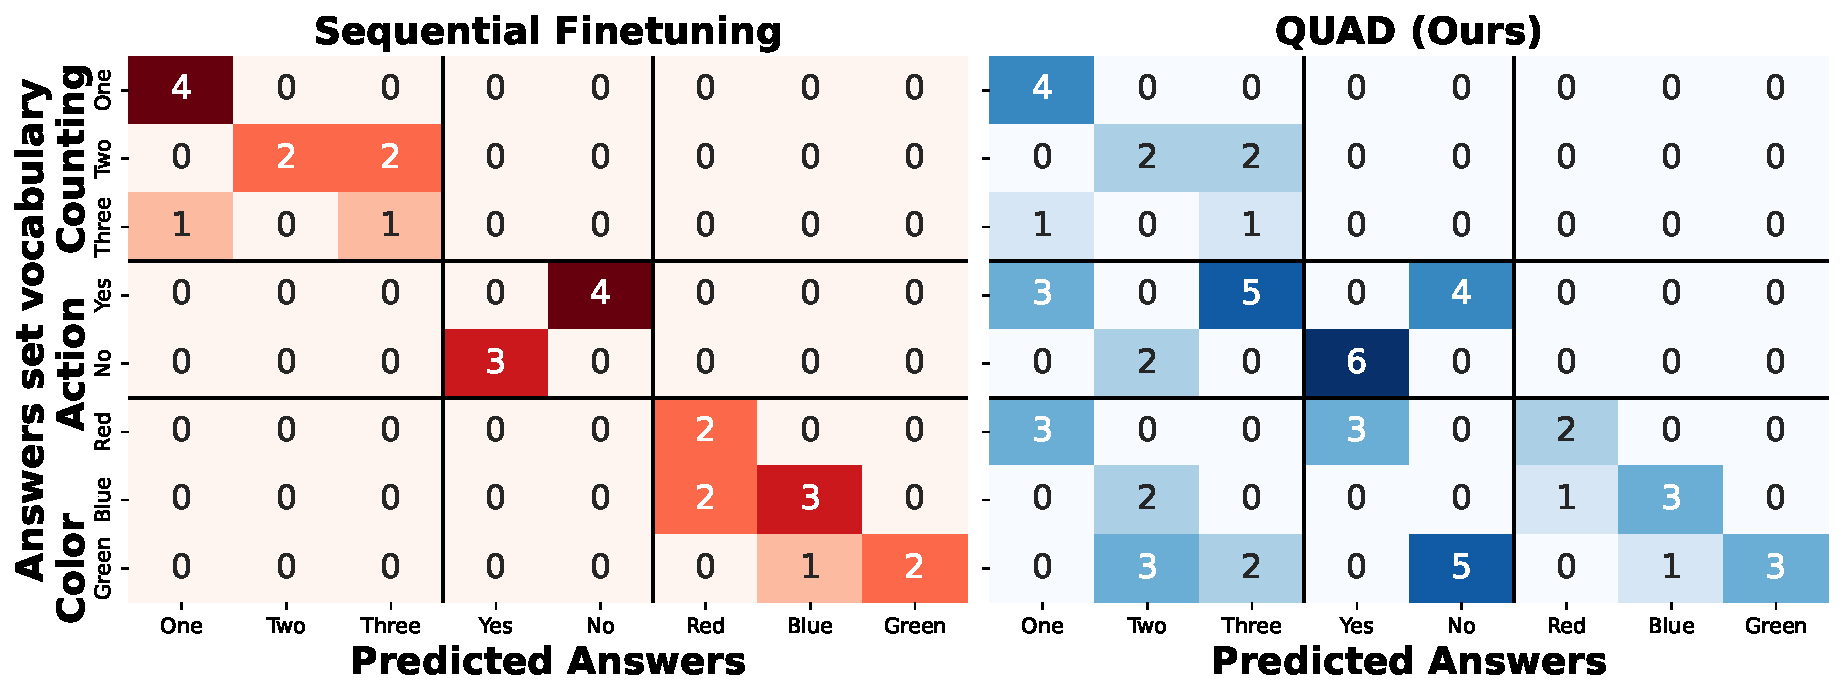
\includegraphics[width=\linewidth]{Figures/confusion_matrices_final.pdf}
    \caption{\textbf{Out-of-Answer-Set Problem in Sequential Finetuning. }Confusion matrices compare Sequential Finetuning (left) and \qstmethodshort{} (right) across three \textit{sequentially} trained tasks: \textit{Counting, Action, and Color} (y-axis: answers set vocabulary, x-axis: predicted answers). Diagonal values indicate model predictions on the current task, while off-diagonal shifts reveal predictions on previous tasks. Sequential Finetuning exhibits, misclassifying past-task questions with responses from the latest task (e.g., counting questions answered with `Yes/No'). \qstmethodshort{} mitigates forgetting, preserving prior knowledge while still adapting to new tasks.}
    \label{fig.out_of_answer_set_problem}
\end{figure}

To address \setting, we propose \textsc{\textbf{QU}estion-only replay with \textbf{A}ttention \textbf{D}istillation} (\textbf{\qstmethodshort{}}), a novel replay framework that balances stability and plasticity using only past questions—no visual data required. Our approach introduces two key contributions, each targeting specific challenges in continual VQA. \textit{First}, we introduce a \textbf{Question-only Replay} mechanism that leverages stored questions from previous tasks to regularize the current model through a strategic selection process that mitigates the \textit{out-of-answer-set problem}, where models overfit to the current task's answer space and consequently misanswer previous queries (see Fig.~\ref{fig.out_of_answer_set_problem}). \textit{Second}, we propose \textbf{Attention Consistency Distillation}, a novel strategy that preserves attention patterns across tasks. It preserves intra-modal (text–text, image–image) and inter-modal (text–image) attention consistency, ensuring the model maintains focus on relevant regions even as it adapts to new information. Extensive experiments on standard VQACL benchmarks (VQAv2 and NExT-QA) demonstrate that \qstmethodshort{} achieves state-of-the-art performance, surpassing both memory-free approaches and rehearsal methods. Notably, \qstmethodshort{} surpasses prior methods that rely on image storage, demonstrating that \textit{storing only questions is sufficient to mitigate forgetting}, validating the practicality of the Question-only Rehearsal (\setting) setting.